\chapter{Aspects techniques}

	\section{Représentation d'un livre}
		\label{sec:representation_livre}

		\subsection{Représentation des noeuds et des liens}



		\subsection{Quelques algorithmes}



	\section{Lecture et écriture d'un livre}

		L'objectif de l'application étant de concevoir un éditeur, il était important de permettre la sauvegarde et la lecture du livre que l'on édite. Le choix du format JSON est rapidement survenue. Premièrement car un fichier d'exemple qui nous a été fournis était sous ce format mais aussi car il s'agit d'une structure simple et très facile à lire. Nous avon alors utilisé GSON, une librairie, conçue par Google, extrêmement simple. Elle permet de retranscrire sous forme d'objet Java un fichier JSON structuré, c'est à dire où l'on distingue très clairement des objets qui se répète.

		Afin de lire un fichier JSON, avec cette librairie, il suffit de concevoir des objets Java avec les même attributs que ceux du fichier à lire ou à écrire. Voici un exemple très court de ce à quoi nos fichiers ressembles :

		\subsection{La structure du JSON}

\begin{lstlisting}[language=json, caption=Exemple de livre très simple, label=lst:exemple_livre]
{
	"prelude": "Vous êtes l'enseignant qui note notre projet",
	"setup": {
		"skills": [],
		"items": [],
		"characters": [],
		"character_creation": []
	},
	"sections": {
		"1" : {
			"text": "Vous être en train d'étudier notre projet",
			"choices": [
				{
					"text": "Mettre une bonne note",
					"section": 3
				},
				{
					"text": "Mettre une mauvaise note",
					"section": 2
				}
			]
		},
		"2": {
			"text": "Les étudiants du projet sont tristes",
			"end_type": "FAILURE"
		},
		"3": {
			"text": "Les étudiants sont satisfait de leur travail",
			"end_type": "VICTORY"
		}
	}
}
\end{lstlisting}

		On retrouve plusieurs éléments différents. On remarque par exemple un attribut "prelude", ainsi que deux grosses parties, "setup" et "sections". Dans la suite, nous détaillerons uniquement les attributs les plus frequemment présents.

		\subsubsection{Setup}

			Commençons par détailler "setup". Ce passage contient toutes les informations générales à notre livre. On y retrouve la liste des compétences ("skills"), la liste des items ("items") et la liste des personnages ("characters"). "character\_creation", lui, détaille toutes les étapes lors de la conception du personnage qui intervient au tout début. Celle-ci permet de sélectionner des skills et items de départ.

			Pour le moment les compétences sont uniquement composé d'un id et d'un nom. Dans une future \maj{} il serait intéressant d'ajouter des propriétés pour connaitre la force ajouté dans un combat, la quantité de soins à rendre par noeuds, par exemple.

\begin{lstlisting}[language=json, caption=Exemple de compétence]
{
	"id": "sixth_sense",
	"name": "Sixième sens"
}
\end{lstlisting}

			Les items peuvent être de différents types : KEY\_ITEM, WEAPON, DEFENSE, MONEY, HEALING. On retrouve pour tous les items un id et un nom ("name"). Pour certains types, des attributs supplémentaires sont présent. Par exemple, un attribut "durability" peut être présent. Il permet de déterminer le nombre d'utilisation maximum d'un item. Un item de type HEALING possède un nombre de pv à rendre ("hp") tandis que ceux type WEAPON possède un montant de dégats ("damage") par exemple.

\begin{lstlisting}[language=json, caption=Exemple d'items]
{
	"id": "backpack",
	"name": "Backpack",
	"item_type": "KEY_ITEM"
},
{
	"id": "healing_potion_4",
	"name": "Potion de soins (4HP)",
	"hp": 4,
	"durability": 1,
	"item_type": "HEALING"
}
\end{lstlisting}

			Concernant les personnages on y retrouve un id, un nom ("name"), un nombre de pv maximum ("hp"), un boolean pour indiquer s'il a beaucoup de chance que ses coups fassent le double des dégats ("double\_damage"), ainsi que "combat\_skill" qui représente le montant de ses dégats.

\begin{lstlisting}[language=json, caption=Exemple de personnage]
{
	"id": "zombie_captain",
	"name": "Zombie Captain",
	"hp": 15,
	"double_damage": true,
	"combat_skill": 2
}
\end{lstlisting}

			Les character character\_creation peuvent être de simple texte ou de type "ITEM" ou "SKILL". On y retrouve les différents skills ou items que l'on peut prendre pour débuter notre aventure ainsi que le nombre que l'on doit en choisir ("amount\_to\_pick").

\begin{lstlisting}[language=json, caption=Exemple de character\_creation]
{
	"text": "Kai Disciplines\n\nOver the centuries, the Kai monks have mastered the skills of the warrior. These skills are known as the Kai Disciplines, [...]",
	"type": "SKILL",
	"skills": [
		"camouflage",
		"hunting",
		"sixth_sense",
		"tracking",
		"healing",
		"weaponskill",
		"mindshield",
		"mindblast",
		"animal_kinship",
		"mind_over_matter"
	],
	"amount_to_pick": 5
}
\end{lstlisting}

		\subsubsection{Sections}

			La partie "sections" est une map qui représente le numéro d'un paragraphe ainsi que le paragraphe associé. Il existe différents types de paragraphes, à choix, à choix aléatoire, avec des combats, terminaux. Tous possède un texte. Les noeuds terminaux possèdent un type de fin ("end\_type") afin savoir si l'on a gagné ou pas (cf : Listing \ref{lst:exemple_livre}). Les noeuds aléatoires eux, possède un attribut "is\_random\_pick" qui vaut true. Pour tous les autres types de noeuds, on retrouve parmis les attributs les plus importants une liste d'items qu'il est possible de prendre, un montant d'item maximum qui peut être pris ("amount\_to\_pick"), des items disponibles à l'achat ("shop").

\begin{lstlisting}[language=json, caption=Exemple de paragraphe]
{
	"text": "The back door opens [...]",
	"items": [
		{
			"id": "gold",
			"amount": 5
		},
		{
			"id": "dagger"
		},
		{
			"id": "seal_hammerdal"
		}
	],
	"amount_to_pick": 2
	"choices": [
		{
			"text": "Return to the tavern.",
			"section": "177"
		},
		{
			"text": "Study the tomb.",
			"section": "24"
		}
	]
}
\end{lstlisting}

			Certains paragraphes peuvent contenir un attribut "combat". Dès lors on peut connaitre le choix en cas de victoire ("win"), de défaite ("loose") ou d'évasion ("evasion). Si l'évasion est possible seulement à partir d'un certains nombre de tour on retrouve alors un attribut nommé "evasion\_round". Pour finir, un attribut "enemies" permet de connaitre les personnages que l'on combat.

\begin{lstlisting}[language=json, caption=Exemple de paragraphe avec des combats]
{
	"text": "The dead zombies lie [...]",
	"combat": {
		"win": {
			"text": "If you win the combat.",
			"section": "309"
		},
		"enemies": [
			"zombie_captain"
		]
	}
}
\end{lstlisting}

			Pour représenter un lien vers un autre paragraphe on retrouve une liste de choix ("choices"). Ils possèdent également un texte qui correspond à l'intititulé du choix, le numéro du paragraphe suivant ("section"), un nombre d'hp à retirer, un nombre d'argent à ajouter ainsi qu'un liste de prérequis ("requirements"). Comme pour les BookNodeLink, il s'agit d'un tableau à deux dimensions. Le premier représente une liste de condition en OU et le second une liste de condition en ET. Enfin, pour les noeuds aléatoire, un poid est également présent ("weight").

\begin{lstlisting}[language=json, caption=Exemple de choix]
{
	"text": "If you have the Kai Discipline of Tracking.",
	"section": "182",
	"hp": -5,
	"requirements":  [
		[
			{
				"id": "tracking",
				"type": "SKILL"
			}
		]
	]
}
\end{lstlisting}

		\subsection{La lecture et l'écriture}

			Du fait que la structure en Json n'est pas identique à celle détaillé dans \nameref{sec:representation_livre} (page \pageref{sec:representation_livre}), nous avons fait des classes intermédiaires pour permettre cette lecture. Celles-ci sont disponibles dans le package \textit{magic\_book/core/file/json} et ne contiennent rien de plus que des getter et setter. Aussi, afin de permettre une convertion entre les classes faites pour représenter un fichier json et celles faites pour être utilisées par l'application, une interface \textit{JsonExportable} existe. Celle ci permet de redéfinir 2 méthodes. L'une renvoyant la classe JSON associé à notre classe actuelle, l'autre permettant à partir d'une classe JSON d'obtenir la classe Java correspondante.

			\begin{figure}[H]
				\centering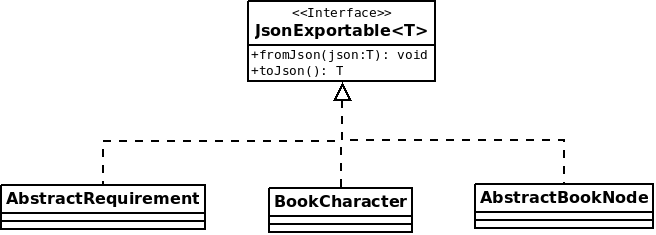
\includegraphics[width=0.66\textwidth, keepaspectratio]{img/json_exportable.png}
				\caption{L'interface JsonExportable et quelques classes qui l'implémentent}
			\end{figure}

			Enfin, les classes BookReader et BookWritter permettent de récupérer toutes les classes JSON intermédiaires pour les regrouper dans le BookJson qui correspond à la structure complète de notre livre. Ces classes sont également une couche d'abstraction à GSON car c'est elles qui se chargent d'écrire le JSON correspondant dans un flux.

			Pour résumer, on peut schématiser ces échanges de telle sorte :

			\begin{figure}[H]
				\begin{center}
					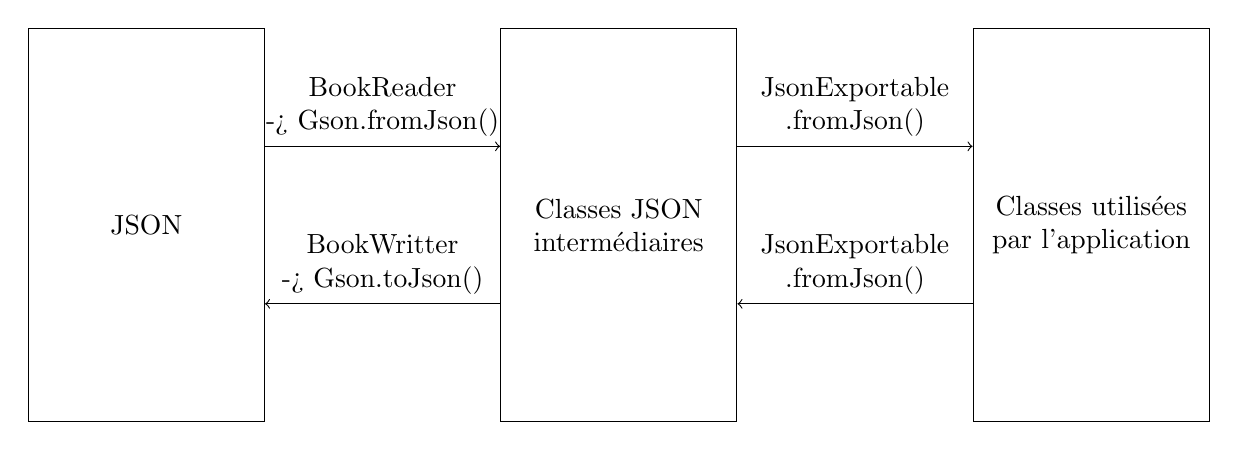
\begin{tikzpicture}
						\node[draw=black, text=black, shape=rectangle, minimum width=3cm, minimum height=5cm] (json) at (0,0) {JSON};
						\node[draw=black, text=black, shape=rectangle, minimum width=3cm, minimum height=5cm, align=center] (json_class) at (6,0) {Classes JSON\\ intermédiaires};
						\node[draw=black, text=black, shape=rectangle, minimum width=3cm, minimum height=5cm, align=center] (class) at (12,0) {Classes utilisées\\ par l'application};

						\draw[->] ([yshift=1cm]json.east) -- node[above, align=center] {BookReader\\ \fontsize{10}{12}\selectfont-> Gson.fromJson()}([yshift=1cm]json_class.west);
						\draw[->] ([yshift=-1cm]json_class.west) -- node[above, align=center] {BookWritter\\ \fontsize{10}{12}\selectfont-> Gson.toJson()}([yshift=-1cm]json.east);

						\draw[->] ([yshift=1cm]json_class.east) -- node[above, align=center] {JsonExportable\\.fromJson()}([yshift=1cm]class.west);
						\draw[->] ([yshift=-1cm]class.west) -- node[above, align=center] {JsonExportable\\.fromJson()}([yshift=-1cm]json_class.east);
					\end{tikzpicture}
				\end{center}
				\caption{Échanges pour la lecture / écriture}
			\end{figure}

	\section{Edition d'un livre}



	\section{Rendre le livre jouable et estimer sa difficulté}
		\underline{Jeu}
		Une classe à été créer se nommant \textbf{Jeu}, permettant de gérer les méthodes de jeu communes entre le \textit{Player} et les \textit{Fourmis}.\\
		Un construteur est d'abord appelé afin d'avoir le livre commun à toute les classes. Puis, celui le mode sélectionner ("Générer la difficulté"" ou "jouer"), on fait appels à la méthode correspondante au player. Une fois quele mode à été cliqué, le livre est alors copié afin de ne pas le modifier dans la classe au cas où. Un BookState, correspondant à la sauvegarde de la partie, est alors créer à partir du BookCharacter généré par le prélude. C'est donc le personnage principal. Si aucun personnages n'est créer, alors un personnage lambda va étre créer afin de pouvoir jouer au jeu.\\
		Une fois le BookState créer et la copie du livre enregistrer, on prend le premier paragraphe et on regarde à quel "noeud" il appartient. Une méthode sera ainsi appeler en fontion du type de noeuds qui prend en charge.\\
		La méthode correspondante au type de noeud s'exécute et renvoie le noeud de "destination", en fonction du choix du player, ou de la mort du player. En effet, ces "noeuds" peuvent faire venir la mort du player en enlevant de la vie par exemple, ou que ce player tombe dans une embuscade... Ces noeuds offre beaucoup de possibilité.\\

		Durant l'exécution de la méthode, et en fonction du player, d'autre méthode externe sont appeler, nottament dans la classe Fourmis ou Player.

	\underline{Interface Player / Foumis}
		Une interface \textbf{InterfacePlayerFoumis} à été créer permettant une mise en commun des codes Player et Fourmis. Ces classes permettent de faire un choix, prendre les items disponibles, créer un personage lambda, aller dans l'inventaire, choisir son ennemis ou encore combatre.\\
		Elles permettrent de d'appeler la même méthode (que cela soit fourmis ou player) au même moment. La méthode sera alors exécuté différément en fonction du player. Cela permet donc une harmonie du code

	\underline{Player}
		La classe \textbf{Player} permet de jouer au jeu en tant que joueur. Elle permet de faire des choix grâce aux Scanner.\\ Cette classe a des méthodes de l'interface, notamment celle de combatChoice qui prend en paramètre le noeud de Combat, le nombre de tour avant l'évasion ainsi que le BookState. Cette méthode permet de choisir nos choix lors de notre tour dans le combat. On peut alors choisir d'attaquer, d'aller dans notre inventaire ou alors de s'évader.\\
		Si on choisi l'inventaire, on va alors dans une autre méthode appelé useInventaire() qui prendre le BookState en parametre. On peut alors utiliser une potion, prendre un objet de défense ou alors une arme. Si l'on choisis un autre choix, cette objet n'est pas utilisable lors d'un combat (comme par exemple de l'argent). Une fois l'objet pris, on retourne dans les choix du combat. On peut alors, soit retourner dans l'inventaire pour prendre un autre objet, soit attaquer ou s'évader.\\
		Si le choix évasion est choisi, un message apparait si le nombre de tour avant l'évasion n'est pas à zero. Si il n'est pas à zéro, un message apparait et il doit refaire un autre choix. Sinon, il va alors dans le noeud de destination qui a été prévu pour l'évasion.\\
		Si le choix attaque est choisi...


	\underline{Fourmis}
